\documentclass[12pt]{article}

% Geometry
\usepackage[margin=1in]{geometry}

% Encoding and fonts
\usepackage[utf8]{inputenc}
\usepackage[T1]{fontenc}
\usepackage[english]{babel}

% Math
\usepackage{amsmath}
\usepackage{amssymb}

% Tables
\usepackage{booktabs}
\usepackage{array}
\usepackage{tabularx}
\usepackage{longtable}

% Figures
\usepackage{graphicx}
\graphicspath{{figures/}}

% References and links
\usepackage[colorlinks=true,linkcolor=blue,citecolor=blue,urlcolor=blue]{hyperref}
\usepackage{natbib}
\bibliographystyle{apa}

% Misc
\usepackage{float}
\usepackage{setspace}
\usepackage{parskip}
\usepackage{microtype}

% Double spacing for review
\doublespacing

% ──────────────────────────────────────────────
\title{21,000 Attempts to Think Differently: A Large-Scale Russian Adaptation of the Divergent Association Task Reveals Practice Resistance and Lexical Predictors of Semantic Creativity}

\author{[Authors blinded for review]}

\date{}

% ──────────────────────────────────────────────
\begin{document}

\maketitle

\noindent\textbf{Running head:} DAT-RU: Practice Resistance and Lexical Predictors

\begin{abstract}
The Divergent Association Task (DAT; Olson et al., 2021) measures verbal creativity by asking participants to name semantically unrelated words. We present DAT-RU, a Russian adaptation deployed as a web application, yielding 21,159 submissions from approximately 1,860 unique users over 50 days. \textbf{Study~1} establishes internal consistency (Cronbach's $\alpha = .90$, split-half $r_{SB} = .70$) but low test--retest reliability ($r = .23$), suggesting divergent association is state-like rather than trait-like. Cross-linguistic calibration shows the 11-point mean score difference between Russian and English samples is largely genuine, not an embedding-model artifact. \textbf{Study~2} models repeated attempts as independent draws from a stable personal distribution: personal bests grow at or below the rate predicted by order statistics, with no evidence of learning or strategic improvement. Marginal returns collapse after 5--10 attempts (125-fold efficiency drop). \textbf{Study~3} identifies category diversity as the strongest predictor of DAT scores ($r = .47$), followed by minimum pairwise distance (the ``weakest link''; $d = 3.89$ between top and bottom performers). A UMAP semantic map reveals that high scorers explore 44\% more semantic territory, while most participants cluster around concrete ``attractor'' words. The theoretical ceiling (110.5) is approached by the best human score (104.8, 95\%) but not by the average participant. Together, these findings characterize the DAT as a reliable single-session measure of semantic exploration breadth that resists strategic gaming but is sensitive to momentary cognitive state.

\medskip
\noindent\textbf{Keywords:} divergent thinking, creativity, semantic distance, Divergent Association Task, word embeddings, practice effects, Russian language, psychometrics
\end{abstract}

\clearpage

% ══════════════════════════════════════════════
\section{Introduction}

Creativity is among the most valued yet most difficult-to-measure human capacities. Traditional assessments of divergent thinking, such as the Alternative Uses Task (AUT; Guilford, 1967) and the Torrance Tests of Creative Thinking (TTCT; Torrance, 1966), require subjective scoring, trained raters, and substantial administration time. These constraints have limited large-scale research on creative cognition.

The Divergent Association Task (DAT; Olson et al., 2021) represents a methodological advance: participants simply name 10 unrelated nouns, and an algorithm computes the mean semantic distance between them using pre-trained word embeddings. The task requires no subjective scoring, takes under three minutes, and can be deployed entirely online. Olson et al.\ demonstrated that DAT scores correlate with established creativity measures ($r = .32$--.51 with AUT flexibility/originality in lab samples; $r = .22$--.34 with Bridge-the-Associative-Gap) and show adequate test--retest reliability over a two-week interval ($r = .73$, $N = 50$; Study~1C). Since its publication, the DAT has been adopted in multiple languages (Chinese: Bai et al., 2024; multilingual: Haase et al., 2025) and research contexts, though at least one replication found weaker convergent validity ($r = .03$ with AUT, $N = 100$; Forthmann \& B\"urkner, 2023), establishing it as a promising but still debated tool for creativity research.

However, several fundamental questions about the DAT remain unaddressed. First, \textbf{how stable are DAT scores across repeated attempts?} The original validation used a single-session design with a controlled two-week retest. In practice, online creativity tests often invite replay---but whether repeated attempts improve performance (through strategy learning) or degrade it (through vocabulary depletion) is unknown. If the DAT is susceptible to gaming, its validity as a trait measure is compromised; if it is resistant, this tells us something fundamental about the nature of divergent association.

Second, \textbf{what lexical and strategic factors predict high DAT scores?} The DAT's algorithm rewards semantic distance, but the cognitive strategies underlying high scores---and whether they can be learned---remain unexplored. Understanding whether high scorers succeed by using rare words, diverse semantic categories, or specific word-selection strategies has implications for both psychometric validity and theories of creative cognition.

Third, \textbf{does the DAT generalize across languages?} Word embeddings differ across languages in their distributional properties, and what constitutes ``semantic distance'' may vary with morphological richness, cultural semantic structures, and corpus characteristics. Cross-linguistic adaptation requires not only translation but calibration of the scoring metric.

We address these questions through DAT-RU, a Russian-language adaptation deployed as a free web application. Viral distribution through social media yielded an unusually large dataset: 21,159 submissions from approximately 1,860 unique users, many of whom returned repeatedly (up to 1,446 attempts). This naturalistic dataset enables analyses that would be impractical in traditional laboratory settings.

We present three studies. Study~1 validates DAT-RU through cross-linguistic calibration and psychometric analysis, revealing a dissociation between high internal consistency and low test--retest reliability that implicates divergent association as a state-like rather than trait-like capacity. Study~2 examines practice effects across thousands of repeated attempts, testing whether performance follows a learning curve or, instead, a random sampling process with diminishing returns. Study~3 identifies the lexical and structural features that distinguish high- from low-scoring word sets, from word frequency and semantic category diversity to the topology of within-set distances.

% ══════════════════════════════════════════════
\section{Methods}

\subsection{The DAT-RU Instrument}

DAT-RU is a browser-based web application implementing a Russian-language version of the Divergent Association Task. Following the original DAT protocol (Olson et al., 2021), participants are presented with 10 input fields and instructed to enter 10 Russian nouns that are ``as semantically distant and unrelated to each other as possible.'' The interface enforces single-word, Cyrillic-only input with real-time validation. A three-minute timer is displayed but not strictly enforced (participants may pause it). The DAT score is computed from the first seven valid words entered, following the original specification that uses the remaining three as a buffer against typographical errors.

\subsection{Embedding Model and Vocabulary}

Word embeddings were obtained from \textbf{navec} (Natasha Project; \url{https://github.com/natasha/navec}), specifically the \texttt{navec\_hudlit\_v1\_12B\_500K\_300d\_100q} model trained on 12 billion tokens of Russian literary texts. The model provides 300-dimensional vectors for approximately 500,000 word forms. We filtered the vocabulary to retain common nouns (excluding proper nouns, surnames, patronymics, toponyms, and abbreviations) using morphological analysis via pymorphy3 (Korobov, 2015). Word forms in any grammatical case or number were mapped to their nominative singular lemma. The character ``yo'' (\textit{\"e}) was normalized to ``ye'' (\textit{e}). The resulting vocabulary comprises 68,841 unique noun lemmas with associated word-form mappings (approximately 400,000 inflected forms).

For browser-based computation, embedding vectors were L2-normalized and quantized from float32 to int8 (multiplied by 127 and clipped to $[-128, 127]$). This quantization introduces approximately 3\% error in cosine distance computations, which we verified to have negligible impact on score rankings (A2 analysis: $r = 1.000$ between int8-computed and float32-computed scores across 200 verified submissions).

\subsection{Score Computation}

The raw DAT score is the mean cosine distance across all 21 unique pairs among the first 7 valid words, multiplied by 100:

\begin{equation}
\text{raw} = \frac{100}{21} \sum_{i=1}^{7}\sum_{j=i+1}^{7}\bigl(1 - \cos(\mathbf{v}_i, \mathbf{v}_j)\bigr)
\label{eq:raw}
\end{equation}

Because the navec embedding space produces a compressed distance distribution relative to the GloVe embeddings used in the original English DAT (median random raw score approximately 87 vs.\ 78), we applied a monotonic power-law calibration:

\begin{equation}
\text{adjusted} = 47.4548 \times \left(\frac{\text{raw}}{100}\right)^{3.3820} + 48.5157
\label{eq:calibration}
\end{equation}

This calibration was derived by fitting to 5,000 random 7-word samples drawn from the navec vocabulary such that the median random score (raw $\approx 87$) maps to 78, matching the English DAT baseline. A separate set of 10,000 random draws was used for ceiling analysis (Section~5.6). All scores reported in this paper are adjusted scores unless otherwise noted. We verified that the nonlinear adjustment preserves the sign, direction, and approximate magnitude of all key correlations (test--retest: $r_{\text{adj}} = .231$ vs.\ $r_{\text{raw}} = .264$; word frequency: $r_{\text{adj}} = -.051$ vs.\ $r_{\text{raw}} = -.058$; time-on-task: $r_{\text{adj}} = .103$ vs.\ $r_{\text{raw}} = .121$).

\subsection{Data Collection}

The application was deployed at [URL redacted for review] and distributed through the first author's Facebook posts beginning February 18, 2026. Distribution was organic: initial posts were shared and reshared within Russian-speaking social networks. No paid promotion or recruitment platforms were used.

Each submission recorded: (a) timestamp (UTC), (b) adjusted DAT score, (c) the seven scoring words (lemmatized), (d) time spent from page load to submission (seconds), and (e) the browser's user-agent string. No personally identifiable information, IP addresses, cookies, or persistent identifiers were collected.

Data collection continued for 50 days (February 18--April 8, 2026), yielding 21,159 submissions. Submission volume showed a viral pattern: a peak of over 4,000 submissions in the first week, decaying to fewer than 100 per day by week~4.

\subsection{User Identification}

In the absence of login-based authentication, the user-agent string served as a proxy for user identity. This is an imperfect method: two individuals using the same device model and browser version are conflated, while a single individual using different devices is split. We identified 1,860 unique user-agent strings, of which 983 (53\%) appeared more than once. Approximately 41\% of records came from user-agents containing specific device identifiers (e.g., ``iPhone17,1'', ``SM-S928B'') where collision probability is low; the remainder came from generic desktop or privacy-masked Android strings where multiple real users may share an identifier. For analyses requiring reliable individual identification (Study~2), we conducted sensitivity analyses restricted to specific user-agent strings and report both full-sample and restricted results. Key findings (test--retest reliability, practice slopes) were stable across confidence tiers (see Supplementary~S4).

\subsection{Descriptive Statistics}

Across all 21,159 submissions: $M = 87.9$, $SD = 7.9$, $Mdn = 89.4$, range $= 48.6$--$104.8$. The distribution was left-skewed (skewness $= -1.65$), with 75\% of scores falling between 84.4 and 93.1. The median time spent was 86 seconds ($M = 99$\,s after excluding outliers below 10\,s and above 1,800\,s). The corpus of submitted words comprised 148,113 word-tokens and 16,952 unique lemmas.

\subsection{Ethical Considerations}

Data were collected anonymously through a publicly available web application. No personally identifiable information was recorded. Participation was voluntary, with no compensation or deception. The study involved no sensitive populations or topics. The anonymized dataset (scores, words, timestamps, and time spent, with user-agent strings removed) will be made publicly available upon publication.

\subsection{Analysis Software}

All analyses were conducted in Python 3.12 using NumPy, SciPy, pandas, statsmodels, matplotlib, and seaborn. UMAP dimensionality reduction used the umap-learn library. Word corpus frequencies were obtained from the wordfreq library (Speer et al., 2018). Mixed-effects models used statsmodels MixedLM. All analysis scripts are available at [repository URL].

% ══════════════════════════════════════════════
\section{Study 1: Cross-Linguistic Validation and Psychometric Properties}

\subsection{Rationale}

Adapting the DAT to a new language raises two questions: (a) are scores comparable across languages, and (b) does the adapted version meet psychometric standards for reliability? We address both through cross-linguistic calibration and internal consistency analysis. Table~\ref{tab:comparison} provides a side-by-side comparison of the key parameters of DAT-RU and the original English DAT.

\begin{table}[htbp]
\centering
\caption{Comparison of DAT-RU and the original English DAT (Olson et al., 2021).}
\label{tab:comparison}
\small
\begin{tabular}{@{}lll@{}}
\toprule
Parameter & DAT (English) & DAT-RU (Russian) \\
\midrule
$N$ (submissions) & 8,914 (Study 1) & 21,159 \\
Recruitment & Amazon MTurk (paid) & Social media (voluntary) \\
Language & English & Russian \\
Words entered / scored & 10 / 7 & 10 / 7 \\
Embedding model & GloVe (Common Crawl, 300d) & navec (hudlit, 300d, int8) \\
Score formula & Mean cosine dist.\ $\times$ 100 & Power-law calibrated to English scale \\
Mean score ($SD$) & 78 (10) & 87.9 (7.9) \\
Score range & $\sim$50--107 & 48.6--104.8 \\
Cronbach's $\alpha$ & Not reported & .899 \\
Split-half ($r_{SB}$) & Not reported & .696 \\
Test--retest $r$ (interval) & .73 (2 weeks, $N = 50$) & .23 (variable, self-selected, $N = 983$) \\
Convergent validity & AUT $r = .32$--.51; BAG $r = .22$--.34 & Not assessed \\
Demographics & Age, gender collected & Not collected \\
Practice effects studied & No & Yes (no learning; i.i.d.\ model) \\
Vocabulary size & Not reported & 68,841 nouns \\
\bottomrule
\end{tabular}
\end{table}

\subsection{Cross-Linguistic Calibration (A1)}

\subsubsection{Method}

We selected the 200 most frequently used words in the DAT-RU dataset and translated them into English using automated translation verified by a bilingual speaker. For each word, we obtained embeddings from both the Russian navec model and the English GloVe model (Common Crawl, 300d; Pennington et al., 2014). We computed pairwise cosine distances for all 19,900 word pairs in both embedding spaces and compared the distance distributions.

To test score equivalence directly, we sampled 1,000 random sets of 7 words from these 200 and computed the raw DAT score for each set in both models.

\subsubsection{Results}

Pairwise distances showed a moderate positive correlation across models (Pearson $r = .664$, Spearman $\rho = .632$, $R^2 = .44$). The two models agree on broad semantic structure but diverge on specific pairs, particularly those affected by polysemy (e.g., the English word ``apple'' is close to ``computer'' due to the corporate entity Apple Inc., an association absent from navec's literary training corpus).

When the same 7-word sets were scored in both models, the Russian model yielded a mean raw score of 90.7, compared to 88.7 for the English model---a difference of only 2.0 points. Crucially, the English GloVe model itself produced scores of approximately 88.7 for these translated Russian words, not the approximately 78 observed in English-speaking samples. This indicates that the 11-point gap between DAT-RU ($M = 87.9$) and the original English DAT ($M \approx 78$) is primarily attributable to word selection ($\approx$9 points), not to embedding model differences ($\approx$2 points). Russian-speaking participants chose more semantically diverse word sets.

\subsection{Internal Consistency (A4)}

\subsubsection{Method}

For all 21,159 submissions, we computed all 21 pairwise cosine distances and assessed internal consistency using: (a) Cronbach's alpha treating the 21 distances as items, and (b) exhaustive split-half reliability across all 35 possible partitions of 7 words into groups of 3 and 4, with Spearman--Brown correction.

\subsubsection{Results}

Cronbach's alpha was .899 (excellent). Exhaustive split-half reliability was $r = .534$ (range across 35 splits: .507--.555), yielding a Spearman--Brown corrected estimate of .696 (95\% CI for corrected $r$: [.689, .701], from 1,000 random-split iterations). These values indicate good internal consistency: within a single session, a participant's seven words form a coherent pattern, and the 21 pairwise distances agree about whether the set is semantically diverse.

However, reliability was strongly score-dependent due to a ceiling effect (Figure~\ref{fig:psychometrics}B). The bottom quintile (most diverse word sets) showed positive within-group reliability ($r = .582$, $\alpha = .933$), while the top four quintiles---compressed into a narrow score range---showed near-zero or negative within-group reliability. This ceiling effect reflects the geometry of high-dimensional cosine distance: once words are drawn from sufficiently distinct categories, further increases in semantic distance become geometrically constrained.

\subsection{Test--Retest Reliability (B1, A3)}

\subsubsection{Method}

For the 983 user-agent strings with two or more submissions, we correlated the score of the first attempt with the score of the second attempt. We conducted sensitivity analyses across user-agent confidence tiers (specific, moderate, generic) to assess the impact of potential user conflation.

\subsubsection{Results}

Test--retest reliability was $r = .231$ ($N = 983$), with a mean score increase from attempt~1 to attempt~2 of 0.61 points ($p = .013$, paired $t$-test). This is substantially lower than the $r = .73$ reported by Olson et al.\ (2021) over a fixed two-week interval with $N = 50$ undergraduates; possible explanations are considered in the Discussion (Section~3.5). The test--retest correlation was remarkably stable across user-agent confidence tiers: specific UAs $r = .225$ ($n = 265$), moderate UAs $r = .253$ ($n = 233$), generic UAs $r = .230$ ($n = 485$). This stability indicates that user-agent collisions do not meaningfully inflate or deflate the reliability estimate.

The dissociation between high internal consistency ($\alpha = .90$, split-half $r_{SB} = .70$) and low test--retest reliability ($r = .23$; Figure~\ref{fig:psychometrics}D) is theoretically informative. If the test were simply noisy, both metrics would be low. Instead, the pattern indicates that the DAT measures reliably at any given moment, but the underlying construct---divergent association ability---fluctuates substantially across occasions. This suggests that verbal divergent thinking, as indexed by the DAT, is more state-like than trait-like, consistent with experience-sampling evidence that daily creative behavior shows substantial within-person variation (ICC $\approx .30$; Silvia et al., 2014) and evidence that divergent thinking performance is sensitive to mood, cognitive load, and environmental context (Baas et al., 2008).

\subsection{Discussion}

DAT-RU demonstrates adequate psychometric properties for a single-session measure: strong internal consistency ($\alpha = .90$) and good split-half reliability ($r_{SB} = .70$). The low test--retest reliability ($r = .23$) contrasts sharply with Olson et al.'s (2021) report of $r = .73$ over a two-week interval with 50 undergraduates. Several factors may contribute to this discrepancy: (a) uncontrolled retest intervals in DAT-RU (minutes to weeks) versus a fixed two-week interval in the original; (b) differing motivational contexts (voluntary replay for entertainment versus paid retest participation); (c) ceiling compression restricting score variability; and (d) genuine state-like fluctuation in semantic exploration ability. The consistency of our estimate across user-agent confidence tiers ($r = .225$--.253) suggests the finding is robust to measurement noise from user identification.

The cross-linguistic calibration indicates that raw DAT scores are not directly comparable across languages. The 11-point mean difference between Russian and English samples reflects real differences in word selection, not embedding-model artifacts. Whether this reflects linguistic, cultural, or demographic factors (the DAT-RU sample was recruited from social media, likely skewing younger and more educated than MTurk samples) remains an open question for future cross-linguistic research.

% ══════════════════════════════════════════════
\section{Study 2: Practice Effects and the Sampling Model of Creativity}

\subsection{Rationale}

DAT-RU's naturalistic deployment produced an unusual dataset: hundreds of users returned voluntarily for repeated attempts, some completing over 1,000 submissions. This enables a test of whether creative performance improves with practice---a question with implications for both test validity (can the DAT be gamed?) and creativity theory (is divergent thinking a learnable skill?).

\subsection{Practice Trajectory Analysis (B1, A3)}

\subsubsection{Method}

We examined score trajectories across attempts using mixed-effects models. For the full sample (983 users with 2 or more attempts, 398 with 5 or more), we fit: score $\sim$ attempt\_number + (1 + attempt\_number $|$ user\_agent) using restricted maximum likelihood. We also examined the distribution of within-user OLS slopes.

\subsubsection{Results}

In the full sample, the fixed effect of attempt number was not significant (slope $= -0.008$, $p = .29$). Within-user OLS slopes were symmetrically distributed around zero (55.3\% positive, 44.7\% negative; mean $= +0.084$, one-sample $t$-test $p = .118$). When restricted to specific user-agent strings (identifiable individuals), a small positive slope emerged ($+0.22$ per attempt, $p = .012$). However, as we show below (Section~4.3), this apparent practice effect is better explained by random sampling dynamics than by genuine learning.

\subsection{The i.i.d.\ Sampling Model (B2)}

\subsubsection{Method}

We tested a null model: each attempt is an independent draw from the user's personal ability distribution, $\text{Normal}(\mu_{\text{user}}, \sigma_{\text{user}})$, with no learning between attempts. Under this model, the personal best after $n$ attempts grows as $E[\max(X_1, \ldots, X_n)]$---a function of order statistics that increases concavely but requires no learning mechanism.

For 121 specific-UA users with 5 or more attempts (69 with 10 or more), we estimated $(\mu, \sigma)$ from all attempts, simulated 1,000 i.i.d.\ replicates, and compared the observed personal-best curve with the i.i.d.\ prediction. Note that estimating $(\mu, \sigma)$ from the same data used for testing introduces a conservative bias: if genuine learning were present, it would inflate $\sigma$, producing an i.i.d.\ prediction with \textit{more} variability than the true null---making the test harder to reject. The fact that observed personal bests fall \textit{below} the i.i.d.\ prediction (Section~4.3 Results) despite this bias strengthens the no-learning conclusion.

\subsubsection{Results}

The i.i.d.\ model fit the data well---in fact, too well (Figure~\ref{fig:practice}A). Observed personal bests grew at or below the rate predicted by random sampling:

\begin{itemize}
    \item At attempt 5: observed PB was 0.59 points \textit{below} the i.i.d.\ prediction ($p = .004$)
    \item At attempt 10: $-1.52$ below ($p < .0001$)
    \item At attempt 20: $-3.09$ below ($p < .0001$)
\end{itemize}

Observed score slopes did not differ from zero (mean $= -0.006$, $p = .95$), and only 6.6\% of users exceeded the 95th percentile of their individual i.i.d.\ null distribution---not significantly above the expected 5\% (binomial $p = .26$). A warm-up test (mean of attempts 4--6 minus mean of attempts 1--3) yielded a negligible difference ($\Delta = -0.21$, $p = .68$).

The sub-i.i.d.\ personal best growth at higher attempt counts suggests mild vocabulary depletion: the finite stock of semantically diverse Russian nouns accessible to a given individual becomes partially exhausted, constraining the generation of novel high-scoring combinations.

\subsection{Optimal Stopping and the Cost of Persistence (E5)}

\subsubsection{Method}

For 57 users with 50 or more attempts, we computed the marginal personal-best gain per attempt and the time invested per additional point.

\subsubsection{Results}

Marginal gains followed the expected order-statistics decay (Figure~\ref{fig:practice}B). Attempt~2 added approximately 3.5 points to the personal best; attempt~5 added 0.6; attempt~10 added 0.2. Time efficiency collapsed accordingly:

\begin{table}[htbp]
\centering
\small
\begin{tabular}{@{}lccc@{}}
\toprule
Attempts & Personal Best & Time Invested & Efficiency \\
\midrule
1--10  & 95.9  & 17 min  & 27.7 pts/hr \\
11--50 & 98.5  & 85 min  & 2.3 pts/hr \\
51+    & 100.5 & 631 min & 0.22 pts/hr \\
\bottomrule
\end{tabular}
\end{table}

This represents a 125-fold efficiency drop between the first 10 and subsequent attempts. Under the i.i.d.\ model with typical user variance, expected marginal gain falls below 0.5 points after attempt~7 and below 0.1 points after attempt~27. Yet the median observed stopping point was 21 attempts---users persisted approximately 2--3 times beyond the point of meaningful return.

\subsection{Discussion}

The dominant pattern across all analyses is clear: \textbf{DAT performance operates as a stationary stochastic process.} Each attempt is effectively an independent draw from a stable personal distribution, with no systematic improvement through practice. This finding is robust to the choice of analysis: mixed-effects models, i.i.d.\ simulation comparisons, and strategy classification all converge on the same conclusion.

The small positive practice slope observed in specific-UA users ($+0.22$ per attempt) does not survive individual-level i.i.d.\ testing. Within-session warm-up effects were present (slope $= +0.39$ per attempt, $p = .014$), but we found no evidence of incubation: between-session transitions ($> 6$ hours, $n = 93$ pairs) showed a nonsignificant score decrease ($\Delta = -0.81$, $p = .22$), and $\log(\text{interval})$ was a negative predictor of score change ($\beta = -0.49$, $p = .047$), though power was limited for overnight intervals ($n = 31$). The absence of incubation effects distinguishes the DAT from insight-based creativity tasks, where sleep and off-task intervals reliably improve performance (Sio \& Ormerod, 2009), and is consistent with the view that the DAT measures divergent \textit{fluency} rather than insight or problem restructuring.

The practical implication is that the DAT is highly resistant to strategic gaming. Feedback and repeated attempts do not meaningfully improve scores. The optimal strategy is 5--10 attempts; beyond this, persistence yields diminishing returns governed entirely by order statistics, not skill acquisition.

% ══════════════════════════════════════════════
\section{Study 3: Lexical Predictors of Creative Performance}

\subsection{Rationale}

If practice does not improve DAT scores, what does differentiate high from low scorers? We examine four classes of lexical predictors: word frequency, semantic category diversity, positional (anchor) effects, and within-set structural topology.

\subsection{Word Frequency (C1)}

\subsubsection{Method}

For each of the 16,952 unique lemmas, we obtained corpus frequency from the wordfreq library (Russian language model; Speer et al., 2018) and computed its mean occurrence in DAT-RU submissions (DAT frequency). For each submission, we computed the mean log corpus frequency of its seven words and correlated this with the DAT score.

\subsubsection{Results}

Participants who used rarer words scored significantly higher ($r = -.239$, $p < .001$; Cohen's $d = 0.66$ comparing top and bottom frequency quartiles: $M = 87.78$ vs.\ 82.92). DAT word frequencies followed Zipf's law but with a flatter slope ($\alpha = 0.76$) than natural language corpora ($\alpha = 1.16$), indicating a more egalitarian word distribution.

Certain concrete, imageable words were massively overrepresented relative to their corpus frequency: ``cat'' (\textit{koshka}) was used 343 times more often than predicted by corpus frequency, followed by ``dog'' (\textit{sobaka}), ``table'' (\textit{stol}), and ``chair'' (\textit{stul}). These ``DAT attractor'' words are prototypically concrete, easily visualized nouns. Conversely, high-frequency abstract words (``time,'' ``year,'' ``matter'') were virtually never used---``semantic blind spots'' reflecting a bias toward imageable over functional semantics.

\subsection{Semantic Category Diversity (C2)}

\subsubsection{Method}

We categorized the 500 most frequent words into 13 semantic categories (Animal, Food, Body, Nature, Home Object, Technology, Place, Abstract, Science, Person, Art/Culture, Emotion, Action/Process). For each submission containing at least 5 categorized words ($n = 3{,}300$), we computed the number of unique categories represented.

\subsubsection{Results}

Category diversity was the strongest single predictor of DAT score ($r = .473$, $p < .001$; Figure~\ref{fig:predictors}A). Mean scores rose sharply with the number of unique categories: 1 category $= 58.0$, 3 categories $= 80.7$, 5 categories $= 84.9$, 6 categories $= 86.1$, with diminishing returns beyond 5 categories.

Top-performing submissions (top 10\%) were characterized by overrepresentation of Abstract ($+16.5\%$ vs.\ bottom 10\%), Action/Process ($+7.4\%$), Person ($+6.1\%$), and Science ($+5.8\%$) categories, while bottom performers overused Home Object ($+11.3\%$), Nature ($+9.7\%$), and Animal ($+8.4\%$) categories. The ``optimal recipe''---the category combination yielding the highest mean score among combinations with at least 10 observations---was Abstract + Action/Process + Food + Nature + Home Object + Person ($M = 100.25$).

Embedding-space analysis confirmed the pattern: the most distant category pairs were Person--Science ($d = 1.037$) and Emotion--Science ($d = 1.034$), while the closest were Emotion--Person ($d = 0.878$) and Nature--Place ($d = 0.897$).

\subsection{Positional and Anchor Effects (C3)}

\subsubsection{Method}

For each submission, we computed each word's mean distance to the other six (positional contribution) and its leave-one-out impact (score change upon removal). We also examined word properties by position: length, corpus frequency, and distance to the set's semantic centroid.

\subsubsection{Results}

A monotonic frequency gradient emerged across positions: position~1 used the most common words (mean log frequency $= -5.44$), declining to position~7 ($-5.64$). First words were shorter (6.31 vs.\ 6.65 characters) and more distant from the set's semantic centroid, consistent with being chosen before the set's thematic structure emerges.

Position~1 made the largest positive contribution to the DAT score (the only position whose removal decreased the score), though all positions contributed roughly proportionally to score prediction ($r = .82$--.88 for each position's isolation metric vs.\ total score).

The most informative analysis concerned the interaction between first-word rarity and completion time. Participants who began with a rare first word (bottom 25\% of corpus frequency) AND completed the task quickly (below-median time) achieved the highest mean scores (0.962 raw), while those who began with a common first word and were fast scored lowest (0.925). Counterintuitively, the rare-word + fast combination outperformed the rare-word + slow combination (0.947), suggesting that rapid access to an unusual first word indexes a stable creative fluency advantage, not effortful deliberation.

\subsection{Within-Set Structural Topology (C4)}

\subsubsection{Method}

For each submission, we computed all 21 pairwise distances and derived structural metrics: standard deviation, coefficient of variation (CV), minimum distance (the ``weakest link''), maximum distance, and range. We classified sets by topology: Uniform (low CV, even distances), Star (one outlier word, rest clustered), Random (high CV, no structure), and Bimodal (two clusters).

\subsubsection{Results}

The minimum pairwise distance---the ``weakest link''---was the most powerful structural predictor beyond the mean. The correlation between minimum distance and DAT score was $r = .764$, and even after controlling for mean distance, the partial correlation remained significant ($r = .156$, $p < .001$). The effect size between top and bottom 5\% of scorers was massive for minimum distance ($d = 3.89$), exceeding even the effect for mean distance ($d = 3.56$). Low-scoring sets almost always contained at least one pair of semantic associates (mean minimum distance $= 0.397$ for bottom 5\% vs.\ 0.821 for top 5\%).

The most common ``bottleneck pairs''---close semantic associates appearing together---were table--chair (31 occurrences), cat--dog (30), male\_dog--female\_dog (23), sea--sun (21), and tomcat--cat (17). A single such pair depressed the overall set score.

Set topology strongly differentiated performance levels. Of all submissions, 90\% were classified as Uniform (mean score $= 89.2$), with the remainder being Random (5.6\%, $M = 75.1$), Star (4.6\%, $M = 77.4$), or Bimodal (0.02\%, $M = 60.9$). Among the top 5\% of scorers, 95.2\% had Uniform topology; among the bottom 5\%, only 20\% were Uniform, with 49\% Random and 31\% Star.

\subsection{Theoretical Ceiling (E1)}

To contextualize human performance, we estimated the maximum achievable DAT score using greedy optimization over the vocabulary. Restricting to common Russian nouns (approximately 180 everyday words), the ceiling was 101.7, achieved by a set spanning maximally distant semantic categories: ``law, curtain, ant, school, silver, airplane, sadness.'' This demonstrates that exotic vocabulary is unnecessary---seven ordinary words from distinct domains suffice for a top-1\% score. The best human score (104.8) exceeded this common-word ceiling, reaching 95\% of the unrestricted theoretical maximum (110.5).\footnote{The unrestricted maximum (110.5) was reached by a set including function words and transliterated foreign names that exploit embedding-space geometry rather than meaningful semantic diversity; we consider the common-word ceiling (101.7) the more interpretable benchmark.} However, the mean human score (87.9) falls closer to the random baseline (adjusted $M = 78.3$ for 10,000 random 7-word draws from the full vocabulary) than to the theoretical maximum, indicating that the average participant captures only a fraction of the available semantic distance.

\subsection{Semantic Map (E3)}

UMAP dimensionality reduction of all 16,952 unique words (colored by mean DAT score and usage frequency; Figure~\ref{fig:umap}) provided a visual synthesis of all lexical findings. The map revealed densely populated ``attractor zones'' around concrete nouns (animals, household objects, nature terms) and sparsely populated territories of abstract, scientific, and process-oriented words. High-scoring participants explored 44\% more unique words (5,979 vs.\ 4,137 for bottom 10\%) and accessed 3,815 words never used by low scorers. This visualization concretizes the mechanism behind practice resistance: most participants repeatedly navigate the same overcrowded semantic neighborhoods, and no amount of repetition expands the territory explored.

\begin{table}[htbp]
\centering
\caption{Summary of lexical predictors of DAT score.}
\label{tab:predictors}
\small
\begin{tabular}{@{}p{4.5cm}cccl@{}}
\toprule
Predictor & $r$ with score & $d$ (top vs.\ bottom) & $N$ & Analysis \\
\midrule
Category diversity (unique categories / 7 words) & $.473^{***}$ & --- & 3,300 & C2 \\
Min pairwise distance (weakest link) & $.156^{***}$ partial\textsuperscript{a} ($.764$ zero-order\textsuperscript{b}) & 3.89 (top vs.\ bottom 5\%) & 21,159 & C4 \\
CV of distances & $-.635^{***}$ & --- & 21,159 & C4 \\
Mean corpus frequency of words & $-.239^{***}$ & 0.66 (Q1 vs.\ Q4) & 21,159 & C1 \\
First-word corpus frequency & $-.18^{***}$ & --- & 21,159 & C3 \\
Set topology (Uniform vs.\ non-Uniform) & --- & Uniform $M = 89.2$ vs.\ Star $M = 77.4$ & 21,159 & C4 \\
Time spent (log seconds) & $.103^{***}$ & --- & 21,121 & D3 \\
\bottomrule
\end{tabular}

\smallskip
\noindent\textit{Note.} \textsuperscript{a}Partial $r$ controlling for mean pairwise distance. \textsuperscript{b}The zero-order $r = .764$ is inflated because minimum distance is a component of the mean that determines the DAT score; the partial $r = .156$ isolates the independent contribution of the weakest link beyond overall distance. $^{***}\, p < .001$.
\end{table}

\subsection{Discussion}

Three converging lines of evidence characterize the lexical basis of DAT performance:

\textbf{The accessibility trap.} Most participants default to concrete, imageable nouns from a handful of dominant categories (animals, household objects, nature). These words are semantically close to each other in embedding space, producing moderate scores. The DAT rewards escape from this accessibility trap---using rarer words ($r = -.24$), diverse categories ($r = .47$), and avoiding any pair of close associates (min distance $d = 3.89$).

\textbf{Uniformity over extremity.} High scores require not one brilliant word but seven consistently distant ones. The ``weakest link'' principle---a single pair of associates drags down the entire score---means that strategic diversity matters more than individual word originality. A set of seven ordinary words from maximally distinct categories (law, curtain, ant, school, silver, airplane, sadness) achieves a score of 101.7, above 99\% of human submissions.

\textbf{Fluency, not deliberation.} The interaction between first-word rarity and speed suggests that high DAT performance indexes a trait-like semantic fluency: the ability to rapidly access diverse regions of semantic space. This fluency is not improved by deliberation (no inverted U-curve for time spent; scores plateau by 90 seconds) or practice (Study~2), reinforcing the view that the DAT measures a stable cognitive property expressed in a state-dependent manner.

% ══════════════════════════════════════════════
\section{General Discussion}

\subsection{Summary of Findings}

Across three studies and 21,159 submissions, DAT-RU reveals a consistent picture of the Divergent Association Task as a measure of semantic exploration breadth. The test is internally consistent ($\alpha = .90$, split-half $r_{SB} = .70$) but produces variable results across occasions (test--retest $r = .23$), suggesting that divergent association is a state-like capacity---reliable within a session but fluctuating across contexts. Practice does not improve performance: repeated attempts follow the statistics of independent random draws, with personal bests converging toward a ceiling governed by order statistics rather than learning. High performance is predicted by lexical diversity (category diversity $r = .47$), word rarity ($d = 0.66$), and structural uniformity (no weak links; $d = 3.89$), while most participants remain trapped in overcrowded semantic neighborhoods of concrete, imageable nouns.

\subsection{Creativity as State: The Reliability Dissociation}

The most theoretically significant finding is the dissociation between internal consistency and temporal stability. If the DAT were simply unreliable, both metrics would be low. Instead, the test captures something real and coherent at each sitting ($\alpha = .90$) that nonetheless varies across occasions ($r = .23$). This places divergent association firmly in the ``state'' end of the state--trait continuum, more variable than typical personality measures ($r \approx .60$--.80) and more variable than other creativity assessments (AUT test--retest $r \approx .56$--.72; Benedek et al., 2013).

We propose that this state-dependence reflects the sensitivity of spontaneous semantic search to momentary cognitive context: current mood (Baas et al., 2008), recent experiences, fatigue, and the stochastic nature of memory retrieval. The i.i.d.\ sampling model (Study~2) provides a formal framework: each attempt is a fresh random walk through semantic space, and the walk's breadth on any given occasion depends on transient activation states rather than fixed ability.

\subsection{The Gamification Paradox}

DAT-RU attracted remarkable engagement: 53\% of users returned for additional attempts, and five users each completed over 600 submissions. Yet this engagement produced no improvement---a ``gamification paradox.'' Users received immediate feedback (their score and a comparison with AI systems), a quantified metric, and social sharing tools---the canonical ingredients of engagement loops. The result was sustained participation without progression.

This paradox is explained by the i.i.d.\ model: because each attempt is statistically independent, the optimal strategy is approximately 5--10 attempts (capturing 95\% of one's personal ceiling via order statistics). Everything beyond this is mathematical futility, with efficiency collapsing 125-fold between the first 10 attempts and subsequent ones. Yet users persisted 2--3 times beyond the optimal stopping point, suggesting that the subjective experience of ``trying harder'' masked the objective reality of diminishing returns.

\subsection{Lexical Accessibility and the Semantic Space}

Study~3 paints a vivid picture of how most people navigate semantic space. The UMAP visualization (Figure~\ref{fig:umap}) shows crowded zones around ``cat,'' ``dog,'' ``table,'' and ``sun''---concrete, imageable nouns that come to mind easily and cluster together in embedding space. High scorers escape these zones by accessing rarer, more abstract, or more domain-specific terms, achieving uniform coverage across semantic space rather than clustering in familiar neighborhoods.

The ``weakest link'' finding has practical implications: a single pair of close associates (cat--dog, table--chair) is sufficient to drag a score from excellent to mediocre. This means that divergent thinking, as measured by the DAT, is as much about \textit{avoiding} automatic associations as it is about \textit{generating} distant ones---a distinction with echoes in inhibitory accounts of creative cognition (Radel et al., 2015).

\subsection{Cross-Linguistic Implications}

The 11-point mean score difference between Russian and English samples is largely genuine rather than artifactual. Whether it reflects linguistic properties (Russian's rich derivational morphology may afford access to more diverse semantic categories), cultural factors, or demographic differences between social-media and MTurk samples remains an important question for future research. Our calibration methodology---comparing same-word-set scores across embedding models---provides a template for cross-linguistic DAT studies, where raw score comparisons are misleading without model-specific normalization.

\subsection{Practical Implications}

For researchers using the DAT as a screening or assessment tool, these findings yield concrete recommendations. A single administration is sufficient: repeated testing does not improve measurement precision and may introduce vocabulary depletion artifacts. If multiple administrations are used (e.g., in pre--post intervention designs), the low test--retest reliability ($r = .23$) should be factored into power analyses, and researchers should expect substantial within-person variability even without any intervention. Cross-linguistic comparisons require embedding-model calibration; raw scores should never be compared across languages without normalization. Finally, the ceiling effect limits the DAT's ability to discriminate among high performers---researchers interested in the upper tail of creative ability may need supplementary measures.

\subsection{Limitations}

Several limitations constrain interpretation. First, \textbf{no external validity measures} (AUT, RAT, Creative Achievement Questionnaire) were collected, preventing assessment of convergent validity. This is especially important given that at least one study has found weak convergent validity for the DAT in English ($r = .03$ with AUT; Forthmann \& B\"urkner, 2023). The semantic category analysis ($r = .47$ between category diversity and score) provides indirect construct validation but does not replace criterion-referenced validation. Second, \textbf{no demographic data} (age, gender, education, native language) were collected, precluding analyses of individual differences. Third, \textbf{user-agent-based identification} is imperfect. While sensitivity analyses showed key findings to be robust across identification confidence tiers, practice-effect analyses are necessarily approximate. Fourth, the sample was drawn from Russian-speaking social media users, likely skewing toward educated, tech-savvy adults, \textbf{limiting generalizability.} Fifth, the \textbf{ceiling effect} (75\% of scores in a narrow range) restricts the test's ability to discriminate among high performers and contributes to score-dependent reliability.

\subsection{Future Directions}

The present findings suggest several avenues for future research. First, a controlled retest study with identified participants and fixed intervals would clarify whether the low test--retest reliability reflects genuine state-like variation or measurement artifacts of the naturalistic design. Second, concurrent administration of DAT-RU with AUT and RAT would establish convergent validity for the Russian adaptation. Third, multilingual embedding models could enable direct cross-linguistic scoring without language-specific calibration; the recent S-DAT framework (Haase et al., 2025), which covers 11 languages including Russian, offers a promising starting point. Fourth, the theoretical ceiling analysis suggests that the DAT's 7-word, mean-cosine-distance scoring metric may be suboptimal: alternative aggregation methods (e.g., minimum distance, trimmed mean) or increased word counts could improve discriminative power in the compressed upper range. Finally, the i.i.d.\ sampling framework could be tested in other creativity tasks to determine whether practice resistance is specific to divergent association or a general property of creative performance.

\subsection{Conclusion}

Twenty-one thousand attempts to think differently reveal a creativity test that resists improvement precisely because it measures something that cannot be practiced. The Divergent Association Task captures the breadth of spontaneous semantic search---a capacity that is internally coherent, state-dependent, and governed by lexical accessibility rather than deliberate strategy. High scores require not one brilliant word but seven consistently distant ones, drawn from across the full breadth of semantic space. Most people never leave the neighborhood of cat, dog, and table.

% ══════════════════════════════════════════════
% Figures
% ══════════════════════════════════════════════

\clearpage

\begin{figure}[htbp]
\centering
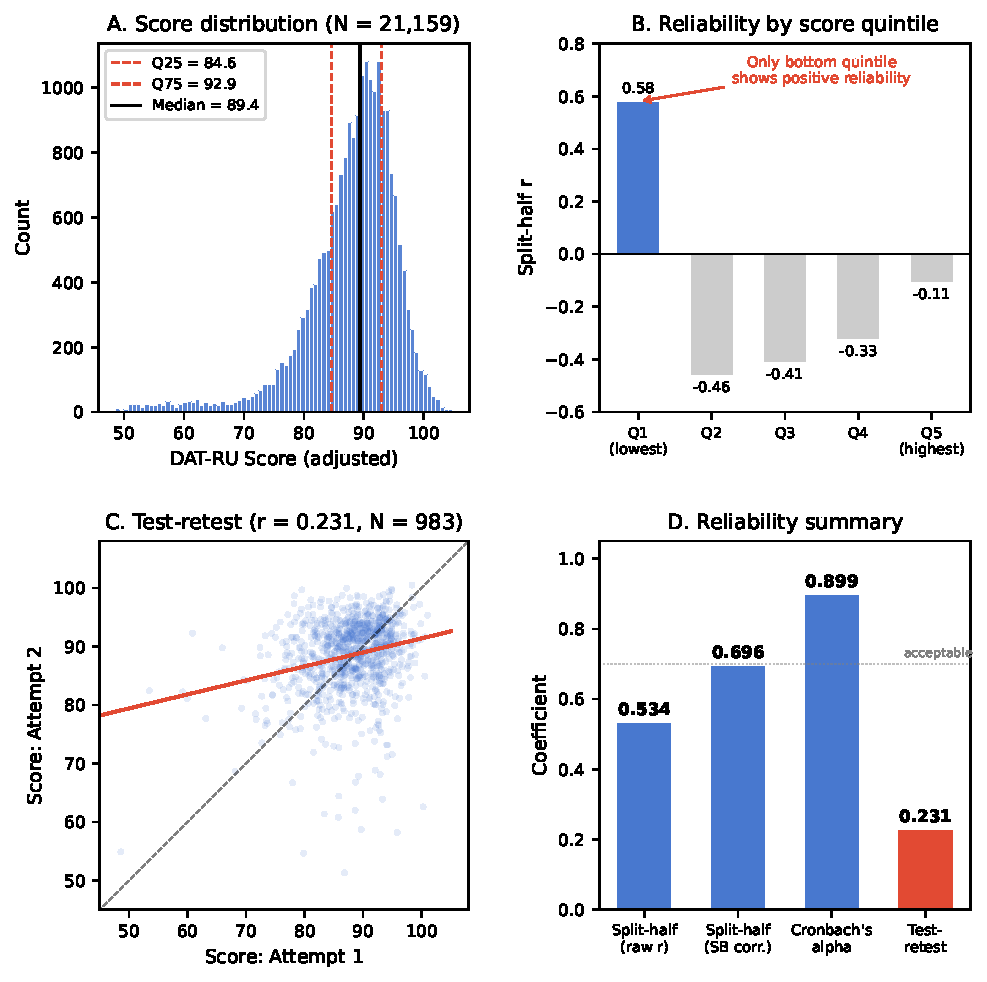
\includegraphics[width=\textwidth]{Figure1_psychometrics.pdf}
\caption{Score distribution and psychometric properties of DAT-RU. (A) Distribution of adjusted DAT scores across 21,159 submissions, showing the left-skewed distribution with 75\% of scores falling between 84.4 and 93.1. (B) Score-dependent reliability: split-half correlation by quintile, illustrating the ceiling effect (positive reliability only in the bottom quintile). (C) Test--retest scatter plot for 983 user-agent strings with two or more attempts, with regression line. (D) Summary of reliability metrics: high internal consistency ($\alpha = .90$, $r_{SB} = .70$) contrasts with low test--retest ($r = .23$).}
\label{fig:psychometrics}
\end{figure}

\begin{figure}[htbp]
\centering
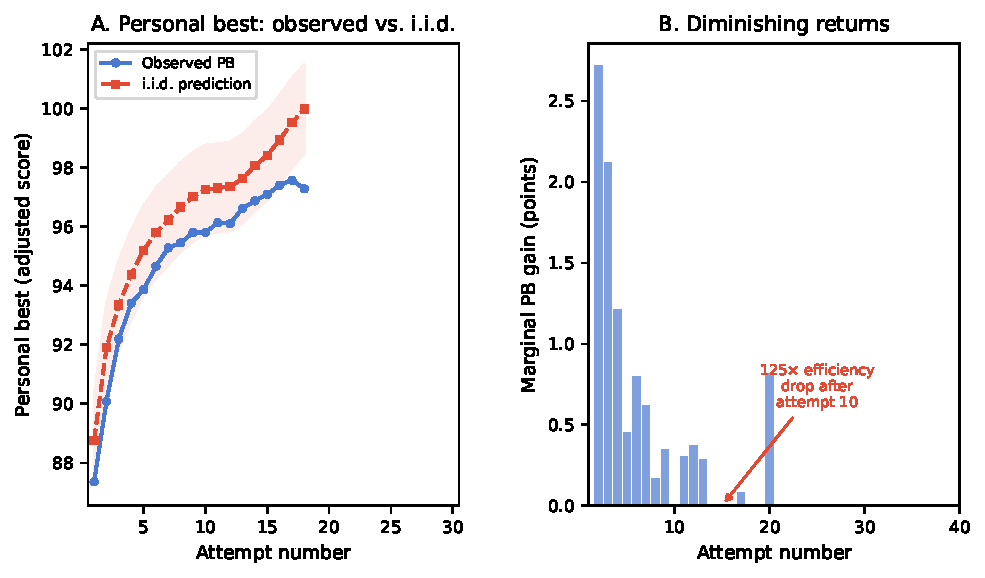
\includegraphics[width=\textwidth]{Figure2_practice.pdf}
\caption{Practice effects and the i.i.d.\ sampling model. (A) Personal-best curves: observed (solid line) versus i.i.d.\ prediction (dashed line) across attempts, with 95\% confidence bands from 1,000 simulations. The observed curve falls at or below the i.i.d.\ prediction, consistent with no learning and mild vocabulary depletion. (B) Optimal stopping: marginal gain per attempt (left axis) and time efficiency in points per hour (right axis), showing the 125-fold efficiency collapse.}
\label{fig:practice}
\end{figure}

\begin{figure}[htbp]
\centering
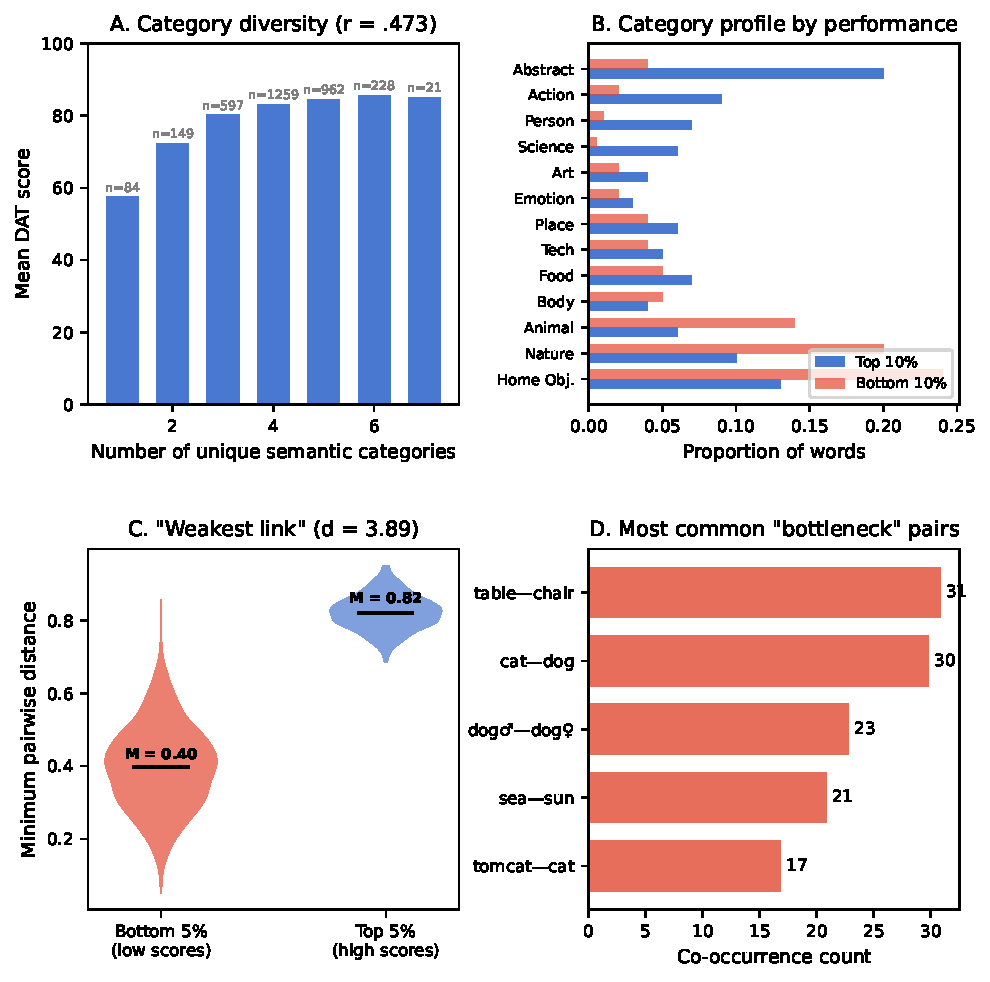
\includegraphics[width=\textwidth]{Figure3_predictors.pdf}
\caption{Lexical predictors of DAT score. (A) Category diversity versus score for 3,300 submissions with 5+ categorized words ($r = .47$). (B) Semantic category profile of top 10\% versus bottom 10\% of scorers, showing overrepresentation of Abstract and Science categories among high scorers. (C) ``Weakest link'' effect: minimum pairwise distance for bottom 5\% ($M = 0.40$) versus top 5\% ($M = 0.82$) of scorers. (D) Most common ``bottleneck'' co-occurring semantic associates that depress set scores.}
\label{fig:predictors}
\end{figure}

\begin{figure}[htbp]
\centering
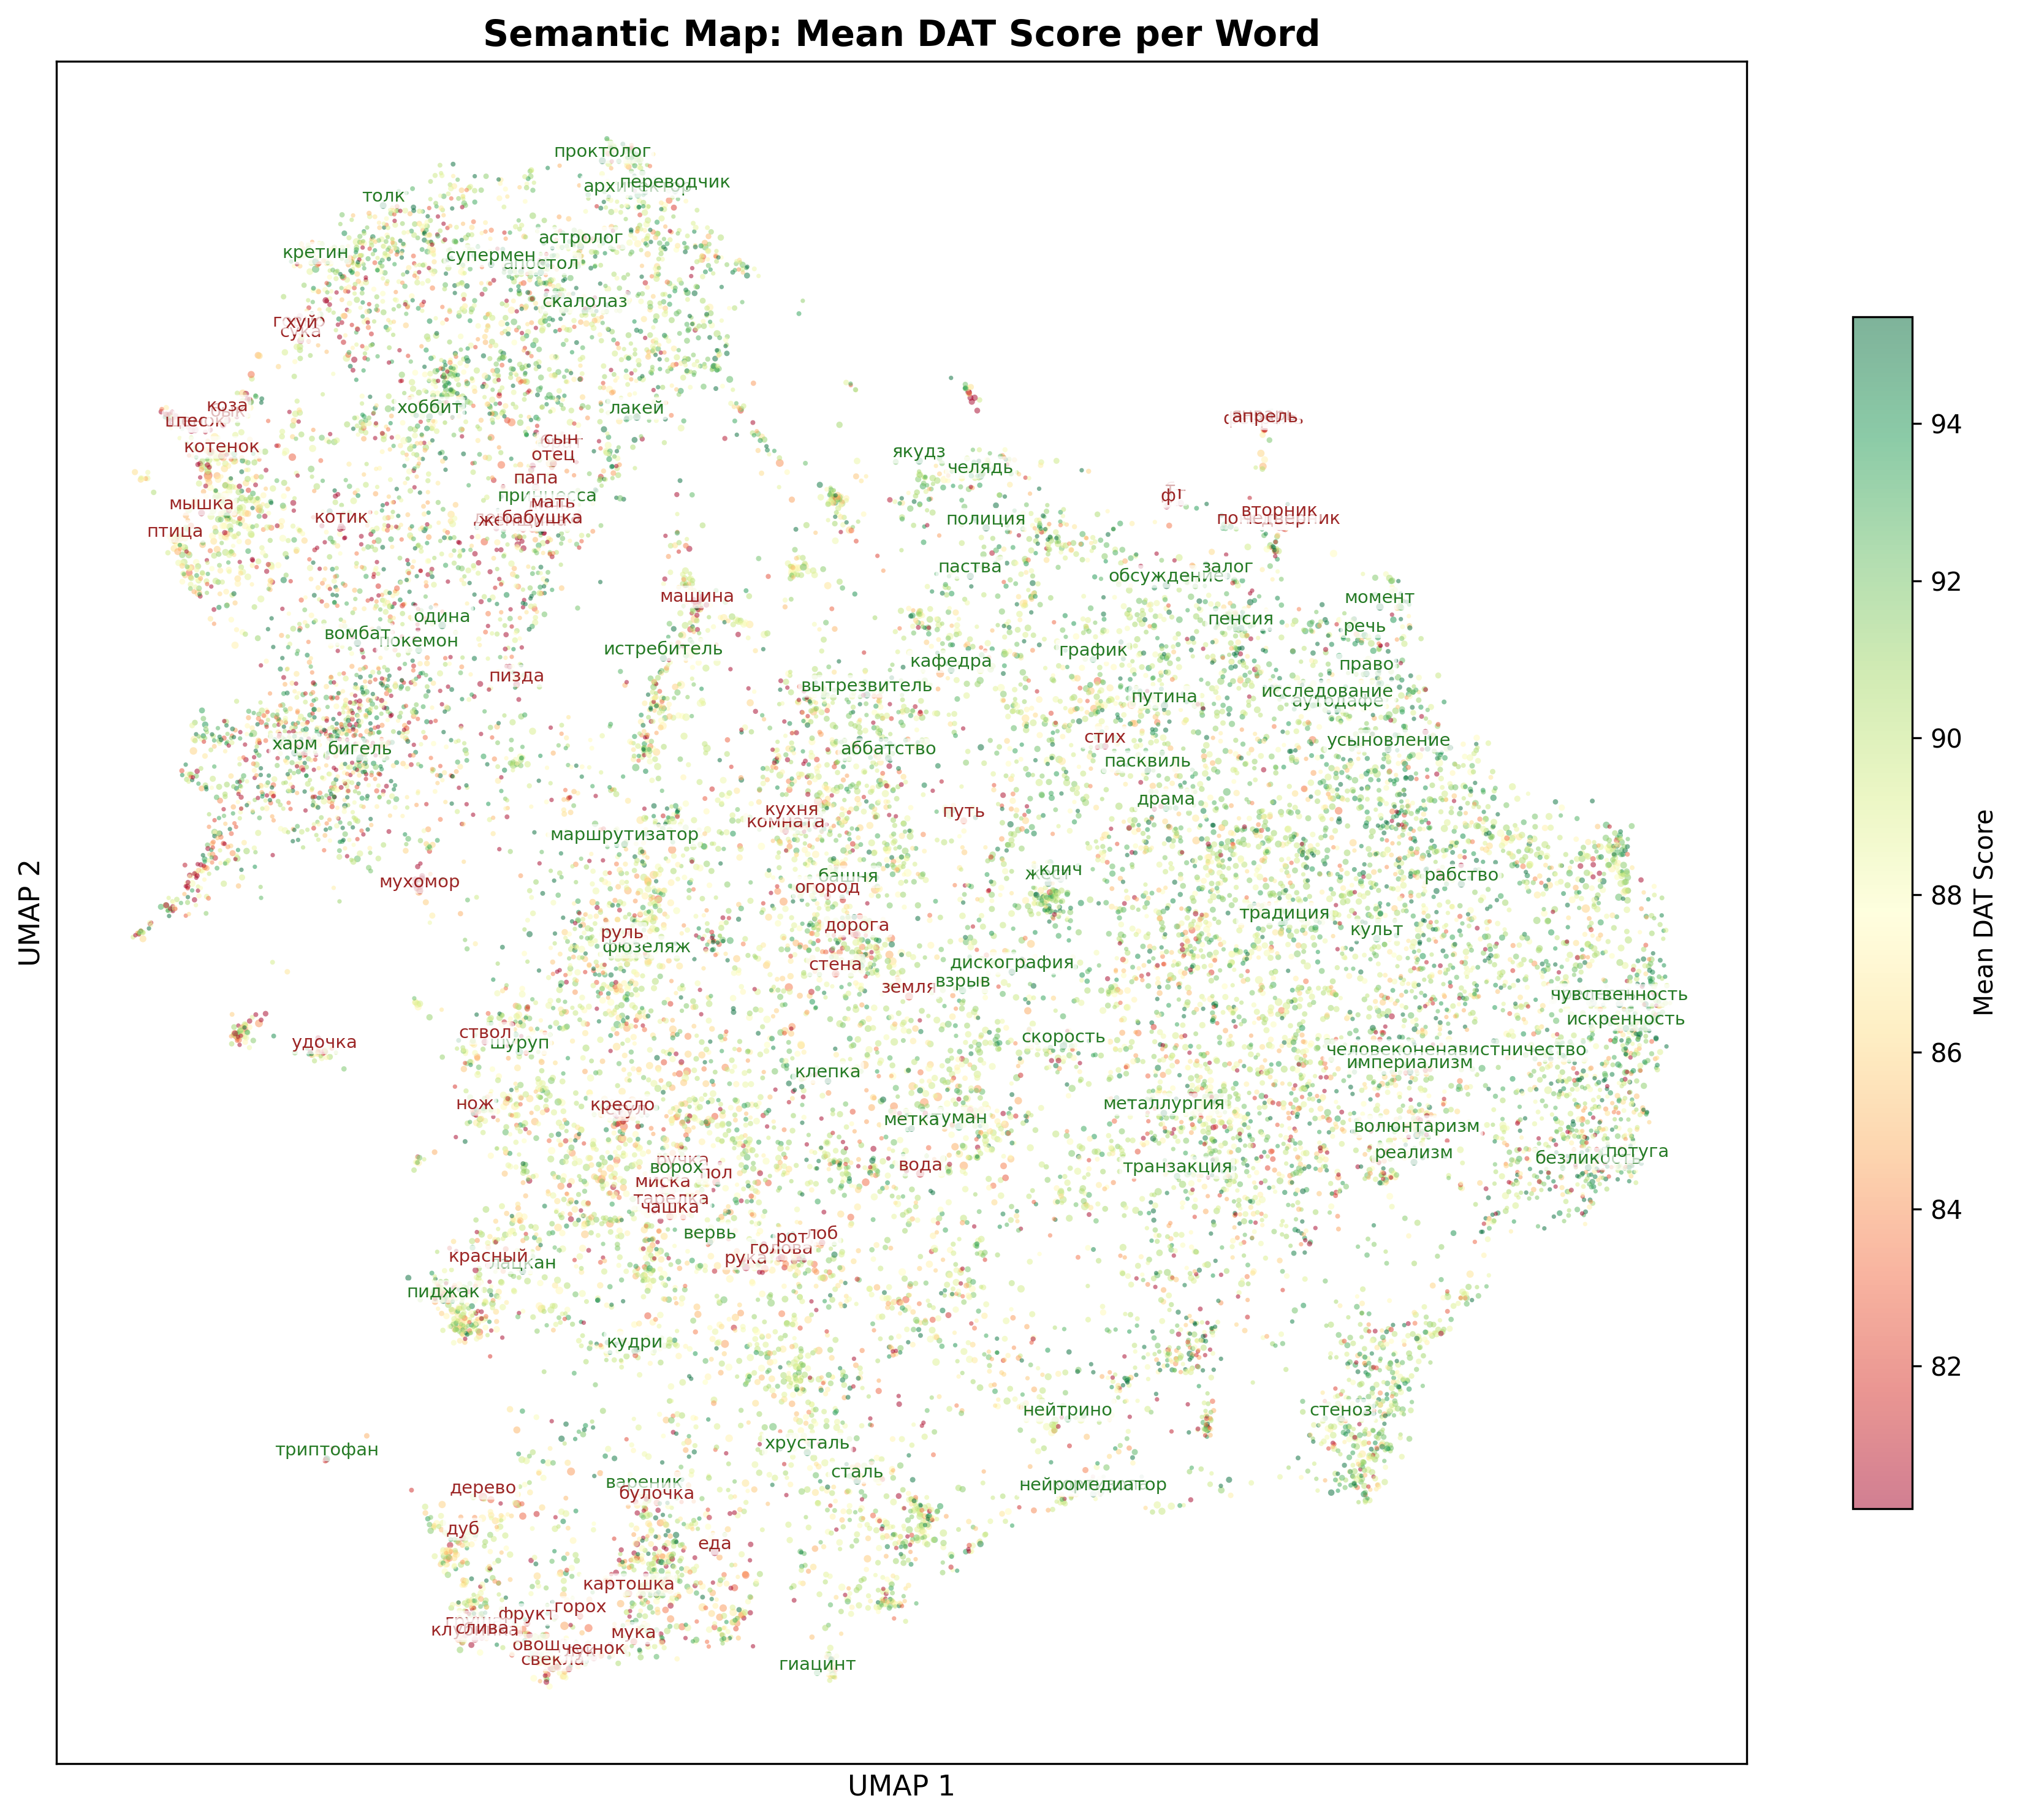
\includegraphics[width=\textwidth]{Figure4_UMAP_semantic_map.png}
\caption{UMAP semantic map of the 16,952 unique words used in DAT-RU submissions, colored by mean DAT score of submissions containing each word. Densely populated ``attractor zones'' around concrete nouns (animals, household objects) are visible in warm colors; high-scoring words (cool colors) occupy sparse peripheral regions of the semantic space.}
\label{fig:umap}
\end{figure}

% ══════════════════════════════════════════════
% References
% ══════════════════════════════════════════════

\clearpage

\begin{thebibliography}{99}

\bibitem[Baas et al., 2008]{baas2008}
Baas, M., De Dreu, C. K. W., \& Nijstad, B. A. (2008). A meta-analysis of 25 years of mood-creativity research: Hedonic tone, activation, or regulatory focus? \textit{Psychological Bulletin, 134}(6), 779--806.

\bibitem[Bai et al., 2024]{bai2024}
Bai, H., Murayama, K., \& Cromley, J. G. (2024). Using the divergent association task to measure divergent thinking in Chinese elementary school students. \textit{Thinking Skills and Creativity, 52}, 101487.

\bibitem[Benedek et al., 2013]{benedek2013}
Benedek, M., M\"uhlmann, C., Jauk, E., \& Neubauer, A. C. (2013). Assessment of divergent thinking by means of the subjective top-scoring method: Effects of the number of top-ideas and time-on-task on reliability and validity. \textit{Psychology of Aesthetics, Creativity, and the Arts, 7}(4), 341--349.

\bibitem[Forthmann \& B\"urkner, 2023]{forthmann2023}
Forthmann, B., \& B\"urkner, P.-C. (2023). The Divergent Association Test lacks convergent validity. \textit{Creativity Research Journal}. Advance online publication.

\bibitem[Guilford, 1967]{guilford1967}
Guilford, J. P. (1967). \textit{The nature of human intelligence.} McGraw-Hill.

\bibitem[Haase \& Hanel, 2023]{haase2023}
Haase, J., \& Hanel, P. H. P. (2023). Artificial muses: Generative artificial intelligence chatbots have risen to human-level creativity. \textit{Journal of Creativity, 33}(3), 100066.

\bibitem[Haase et al., 2025]{haase2025}
Haase, J., Hanel, P. H. P., \& Pokutta, S. (2025). S-DAT: A multilingual, GenAI-driven framework for automated divergent thinking assessment. In \textit{Proceedings of the AAAI/ACM Conference on AI, Ethics, and Society}. arXiv:2505.09068.

\bibitem[Hubert et al., 2024]{hubert2024}
Hubert, K. F., Awa, K. N., \& Zabelina, D. L. (2024). The current state of artificial intelligence generative language models is more creative than humans on divergent thinking tasks. \textit{Scientific Reports, 14}, 3440.

\bibitem[Kim, 2006]{kim2006}
Kim, K. H. (2006). Can we trust creativity tests? A review of the Torrance Tests of Creative Thinking (TTCT). \textit{Creativity Research Journal, 18}(1), 3--14.

\bibitem[Korobov, 2015]{korobov2015}
Korobov, M. (2015). Morphological analyzer and generator for Russian and Ukrainian languages. \textit{Communications in Computer and Information Science, 542}, 320--332.

\bibitem[Olson et al., 2021]{olson2021}
Olson, J. A., Nahas, J., Chmoulevitch, D., Cropper, S. J., \& Webb, M. E. (2021). Naming unrelated words predicts creativity. \textit{Proceedings of the National Academy of Sciences, 118}(25), e2022340118.

\bibitem[Pennington et al., 2014]{pennington2014}
Pennington, J., Socher, R., \& Manning, C. D. (2014). GloVe: Global vectors for word representation. In \textit{Proceedings of the 2014 Conference on Empirical Methods in Natural Language Processing (EMNLP)} (pp.\ 1532--1543).

\bibitem[Radel et al., 2015]{radel2015}
Radel, R., Davranche, K., Fournier, M., \& Dietrich, A. (2015). The role of (dis)inhibition in creativity: Decreased inhibition improves idea generation. \textit{Cognition, 134}, 110--120.

\bibitem[Silvia et al., 2014]{silvia2014}
Silvia, P. J., Beaty, R. E., Nusbaum, E. C., Eddington, K. M., Levin-Aspenson, H., \& Kwapil, T. R. (2014). Everyday creativity in daily life: An experience-sampling study of ``little c'' creativity. \textit{Psychology of Aesthetics, Creativity, and the Arts, 8}(2), 183--188.

\bibitem[Sio \& Ormerod, 2009]{sio2009}
Sio, U. N., \& Ormerod, T. C. (2009). Does incubation enhance problem solving? A meta-analytic review. \textit{Psychological Bulletin, 135}(1), 94--120.

\bibitem[Speer et al., 2018]{speer2018}
Speer, R., Chin, J., \& Havasi, C. (2018). ConceptNet 5.5: An open multilingual graph of general knowledge. In \textit{Proceedings of the AAAI Conference on Artificial Intelligence, 31}(1).

\bibitem[Torrance, 1966]{torrance1966}
Torrance, E. P. (1966). \textit{The Torrance Tests of Creative Thinking: Norms-technical manual.} Personnel Press.

\end{thebibliography}

% ══════════════════════════════════════════════
% Appendix: Supplementary Materials
% ══════════════════════════════════════════════

\clearpage
\appendix
\section{Supplementary Materials}

\subsection{S1. Time-on-Task and Device Effects (D3)}

Time spent showed a logarithmic relationship with score: performance improved up to approximately 90 seconds, then plateaued. There was no inverted U-curve; additional time beyond 90 seconds did not impair performance (LOWESS peak at 133 seconds, but the gain from 63 to 133 seconds was only 0.7 points). Median time per word was 12.3 seconds.

Device type (Android 47\%, iPhone 31\%, Desktop 21\%) showed minimal score differences ($F = 4.55$, $p = .01$; maximum difference of 0.4 points between Android and Desktop). Time spent did not differ across devices.

Weekend submissions scored slightly higher than weekday (88.5 vs.\ 87.5, $p < .001$), likely reflecting selection effects (more leisure-time engagement) rather than circadian creativity effects. No robust time-of-day pattern was observed after controlling for repeat users.

\subsection{S2. Temporal Dynamics}

Submission volume peaked in the first week ($> 4{,}000$ submissions on the peak day) and decayed to $< 100$/day by week~4, consistent with viral social media dynamics. Later-arriving users scored slightly lower (Spearman $\rho = -.12$, $p < .001$), possibly reflecting broader audience reach beyond the initial, more engaged cohort.

\subsection{S3. Example Word Sets}

Table~\ref{tab:examples_top} presents example submissions illustrating high, typical, and low DAT scores, with English translations.

\begin{table}[htbp]
\centering
\caption{Top-scoring sets (score $> 104$).}
\label{tab:examples_top}
\small
\begin{tabular}{@{}clp{7cm}c@{}}
\toprule
Score & Words (Russian) & Translation & Time \\
\midrule
104.8 & \parbox[t]{4cm}{\raggedright vombat, stal', issledovanie, drama, shepot, pidzhak, svyatki} & wombat, steel, research, drama, whisper, jacket, Yuletide & 51\,s \\
104.3 & \parbox[t]{4cm}{\raggedright prelest', neyromediator, kapot, imperializm, usynovlenie, chelyad', kanonada} & charm, neurotransmitter, hood, imperialism, adoption, servants, cannonade & 81\,s \\
104.2 & \parbox[t]{4cm}{\raggedright chelovekonenavist\-nichestvo, moment, triptofan, zhizn', fazenda, yuan', plastika} & misanthropy, moment, tryptophan, life, hacienda, yuan, surgery & 75\,s \\
\bottomrule
\end{tabular}
\end{table}

\begin{table}[htbp]
\centering
\caption{Typical sets (score $\approx 89$).}
\label{tab:examples_typical}
\small
\begin{tabular}{@{}clp{7cm}c@{}}
\toprule
Score & Words (Russian) & Translation & Time \\
\midrule
89.1 & \parbox[t]{4cm}{\raggedright styuardessa, khloroform, prityazhenie, algoritm, skalolaz, zanuda, muraved} & stewardess, chloroform, gravity, algorithm, climber, bore, anteater & 119\,s \\
89.1 & \parbox[t]{4cm}{\raggedright ryukzak, khrizantema, kopyto, kley, lyagushka, solntse, banka} & backpack, chrysanthemum, hoof, glue, frog, sun, jar & 57\,s \\
89.1 & \parbox[t]{4cm}{\raggedright kot, rabota, gel', pal'ma, vosk, struna, molekula} & cat, work, gel, palm, wax, string, molecule & 153\,s \\
\bottomrule
\end{tabular}
\end{table}

\begin{table}[htbp]
\centering
\caption{Bottom-scoring sets (score $< 50$).}
\label{tab:examples_bottom}
\small
\begin{tabular}{@{}clp{7cm}c@{}}
\toprule
Score & Words (Russian) & Translation & Time \\
\midrule
48.6 & \parbox[t]{4cm}{\raggedright yanvar', fevral', mart, aprel', may, iyun', iyul'} & January, February, March, April, May, June, July & 27\,s \\
48.6 & \parbox[t]{4cm}{\raggedright yanvar', dekabr', fevral', mart, aprel', sentyabr', oktyabr'} & January, December, February, March, April, September, October & 116\,s \\
\bottomrule
\end{tabular}

\smallskip
\noindent\textit{Note.} The bottom-scoring sets illustrate the ``weakest link'' principle: listing words from a single semantic category (months) produces uniformly small pairwise distances. The 116-second example suggests a deliberate (not rushed) attempt that still failed due to category restriction.
\end{table}

\subsection{S4. User-Agent Sensitivity Analysis}

User-agent strings were classified into three confidence tiers based on device model specificity: Specific (41\% of records; identifiable device model, low collision risk), Moderate (26\%; partial device information), and Generic (33\%; desktop browsers or privacy-masked Android devices, higher collision risk). Key findings were stable across tiers: test--retest $r = .225$ (specific), .253 (moderate), .230 (generic). Among users with 50+ attempts, 65\% of generic-UA ``heavy users'' showed suspicious temporal patterns (24-hour activity spread) consistent with multiple real individuals sharing a user-agent string. Full details in analysis\_A3.

\subsection{S5. Data and Code Availability}

The anonymized dataset (scores, words, timestamps, time spent) and all analysis scripts are available at [repository URL]. User-agent strings are excluded to protect participant privacy.

\end{document}
